\section{Ứng dụng hỏi đáp hợp đồng (Assignment 3)}

Hệ thống hỏi đáp (QA System) trong đồ án này không chỉ đơn thuần là một chatbot RAG (Retrieval-Augmented Generation) cơ bản. Hệ thống được thiết kế theo kiến trúc "Legal Search Architect" - một quy trình truy xuất đa tầng kết hợp giữa hiểu biết ngữ cảnh của LLM và các thông tin cấu trúc (NER, SRL, Intent) đã trích xuất ở Assignment 1 và 2.

\subsection{Kiến trúc hệ thống RAG đa tầng}

Thay vì đưa trực tiếp câu hỏi của người dùng vào cơ sở dữ liệu vector, hệ thống thực hiện một quy trình gồm 3 giai đoạn chính:

\begin{enumerate}
    \item \textbf{Giai đoạn 1 - Lập kế hoạch truy vấn (Search Blueprint):} Sử dụng Gemini để phân tích câu hỏi và tạo ra một "bản thiết kế" tìm kiếm dưới dạng JSON, bao gồm các bộ lọc về thực thể, ý định và vai trò ngữ nghĩa.
    \item \textbf{Giai đoạn 2 - Truy xuất mục tiêu (Targeted Retrieval):} Thực hiện lọc cứng (Hard Filter) trên metadata của ChromaDB và tái xếp hạng (Re-rank) bằng thuật toán chấm điểm SRL Heuristic.
    \item \textbf{Giai đoạn 3 - Sinh câu trả lời có trích dẫn:} Kết hợp ngữ cảnh đã tinh lọc để Gemini tổng hợp câu trả lời cuối cùng theo phong cách văn bản pháp quy.
\end{enumerate}

\begin{figure}[H]
    \centering
    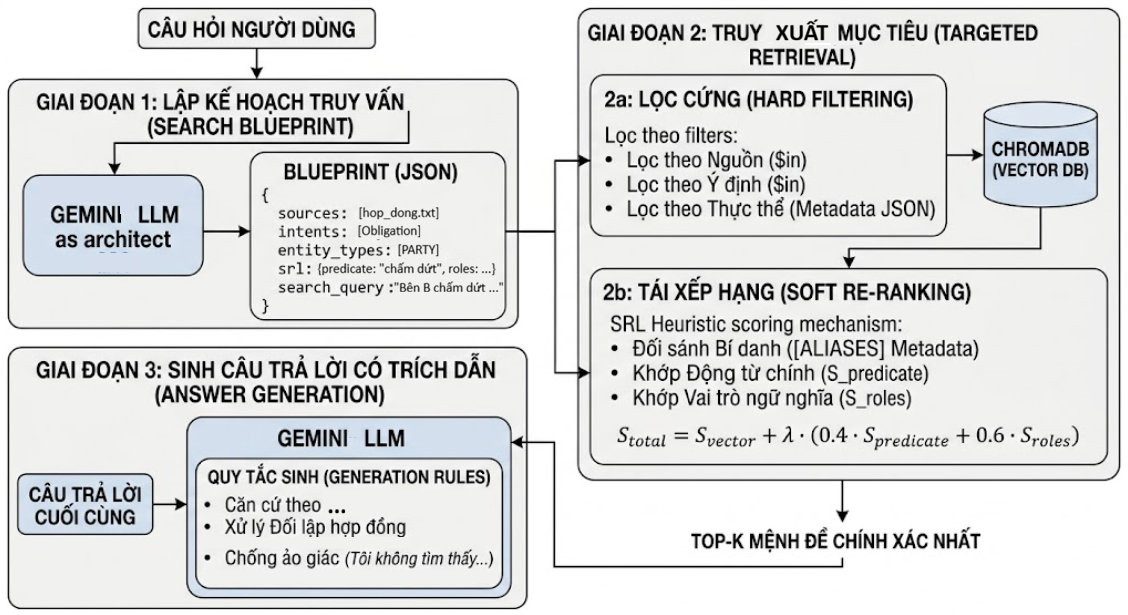
\includegraphics[width=1.0\textwidth]{Image/rag_pipeline.png}
    \caption{Quy trình truy xuất và xử lý của hệ thống QA.}
    \label{fig:rag_flow}
\end{figure}

\subsection{Khối truy xuất tri thức nâng cao (Legal Retriever)}

Đây là thành phần cốt lõi đảm bảo tính chính xác và giảm thiểu hiện tượng "ảo giác". Cơ chế lọc được chia làm hai loại: Lọc cứng (Hard Filter) và Lọc mềm (Soft Re-ranking).

\subsubsection{Cơ chế tạo Search Blueprint bằng Gemini}

Khi nhận câu hỏi, hệ thống gửi một Prompt đặc biệt tới Gemini (xem tại \texttt{src/qa/generator.py}) để yêu cầu mô hình đóng vai trò một kiến trúc sư tìm kiếm. 

\textbf{Ví dụ:} 
\begin{itemize}
    \item \textbf{Câu hỏi:} "Điều gì xảy ra nếu Công ty ABC chậm thanh toán?"
    \item \textbf{Blueprint (JSON) tạo bởi Gemini:}
\end{itemize}

\begin{verbatim}
{
  "sources": ["hop_dong_thue_nha.txt"],
  "intents": ["Termination Condition", "Obligation"],
  "entity_types": ["PARTY", "PENALTY"],
  "srl": {
    "predicate": "thanh toán",
    "roles": {"AGENT": "Công ty ABC", "CONDITION": "chậm"}
  },
  "search_query": "chậm thanh toán xử phạt chấm dứt hợp đồng"
}
\end{verbatim}

\subsubsection{Chiến lược lọc đa tầng (Multi-stage Filtering)}

Dựa trên Blueprint, hàm \texttt{retrieve} trong \texttt{src/qa/ retriever.py} thực hiện lọc theo thứ tự:

\begin{enumerate}
    \item \textbf{Lọc theo Nguồn (Source Filter) và Ý định (Intent Filter):} Đây là bước lọc cứng ngay tại tầng cơ sở dữ liệu vector (ChromaDB) bằng toán tử \texttt{\$in}. Hệ thống chỉ lấy các mệnh đề thuộc đúng file hợp đồng và có ý định pháp lý phù hợp (ví dụ: chỉ tìm trong các câu mang tính "Nghĩa vụ" hoặc "Điều kiện chấm dứt").
    \item \textbf{Lọc theo Thực thể (Entity Filter):} Hệ thống duyệt qua Metadata \texttt{entities} (đã được lưu dưới dạng chuỗi JSON ở bước Ingest, ví dụ: chỉ những mệnh đề chứa loại thực thể như \texttt{PARTY} hoặc \texttt{MONEY} được yêu cầu mới được giữ lại).
\end{enumerate}

\subsubsection{Thuật toán chấm điểm SRL và Tái xếp hạng (Soft Re-ranking)}

Mặc dù Lọc Cứng (Hard Filter) giúp thu hẹp không gian tìm kiếm, độ chính xác của các câu lệnh truy vấn ngữ nghĩa truyền thống (chỉ dựa vào vector embedding) thường bị giảm sút do hiện tượng "tương đồng bề mặt" (surface similarity). Ví dụ, câu hỏi "Ai trả tiền cho Bên A?" và mệnh đề "Bên A trả tiền cho Bên B" có độ tương đồng vector rất cao do trùng lặp từ vựng, nhưng lại mang ý nghĩa trái ngược nhau. 

Để giải quyết vấn đề này, hệ thống áp dụng kỹ thuật \textbf{Tái xếp hạng (Re-ranking) dựa trên Gán nhãn Vai trò Ngữ nghĩa (SRL)}. Hàm \texttt{\_calculate\_srl\_score} (trong \texttt{src/qa/ retriever.py}) đóng vai trò tinh chỉnh điểm số của các ứng viên dựa trên mức độ khớp của từng thành phần cấu trúc (Vị ngữ và các Vai trò).

Thuật toán chấm điểm SRL ($S_{srl}$) được cấu thành từ hai phần chính: Điểm Vị ngữ ($S_{predicate}$) và Điểm Vai trò ($S_{roles}$).

\paragraph{Chấm điểm Vị ngữ ($S_{predicate}$ - Trọng số 0.4):}
Đầu tiên, hệ thống so sánh hành động chính (Predicate) được yêu cầu trong \textit{Search Blueprint} ($P_{query}$) với Vị ngữ đã được trích xuất sẵn trong Metadata của mệnh đề ($P_{doc}$). Các mức độ khớp được xử lý theo quy tắc giảm dần:
\begin{itemize}
    \item \textbf{Khớp tuyệt đối (Exact Match):} Nếu $P_{query}$ hoàn toàn trùng khớp với $P_{doc}$, $S_{predicate}$ đạt tối đa $1.0$ (tương đương $+0.4$ vào tổng điểm).
    \item \textbf{Khớp một phần (Substring Match):} Nếu một từ nằm trong từ còn lại (ví dụ: "thanh toán" và "thanh toán tiền"), hệ thống ghi nhận điểm $0.625$ (tương đương $+0.25$).
    \item \textbf{Khớp ngữ nghĩa (Semantic Embedding Match):} Nếu không có sự trùng lặp từ vựng, hệ thống tính toán Cosine Similarity giữa vector embedding của $P_{query}$ và $P_{doc}$ (sử dụng cùng mô hình \textit{Vietnamese-SBERT}). 
    \begin{equation}
        \text{CosSim}(P_{query}, P_{doc}) = \frac{E_{P_{query}} \cdot E_{P_{doc}}}{\|E_{P_{query}}\| \|E_{P_{doc}}\|}
    \end{equation}
    Nếu $\text{CosSim} > 0.6$, điểm $S_{predicate}$ được tỷ lệ hóa tuyến tính trong khoảng $[0, 0.5]$ (tương đương $+0.2$ vào tổng). Nếu Cosine Similarity thất bại, thuật toán lui về đối sánh mức độ trùng lặp từ vựng (Jaccard Similarity).
\end{itemize}

\paragraph{Cơ chế Đối sánh Bí danh (Alias Matching) cho Vai trò ($S_{roles}$ - Trọng số 0.6):}
Sau khi xác định mức độ khớp của hành động, hệ thống đối chiếu từng vai trò ngữ nghĩa (như \texttt{AGENT}, \texttt{THEME}, \texttt{RECIPIENT}) giữa \textit{Blueprint} và \textit{Metadata} của mệnh đề. Đây là bước quyết định xem "ai làm gì với ai" có thực sự trùng khớp hay không.

Khó khăn lớn nhất trong hợp đồng là tính đa danh xưng. Một thực thể có thể được gọi bằng nhiều cách: "Công ty ABC", "Bên A", hoặc "Bên cho thuê". Nếu chỉ so sánh chuỗi thông thường, "Công ty ABC" và "Bên A" sẽ trả về điểm $0$, dẫn đến việc loại bỏ nhầm mệnh đề quan trọng.

Để khắc phục, hệ thống tận dụng thẻ \texttt{[ALIASES]} được Gemini trích xuất ở khâu tiền xử lý (ví dụ: \texttt{[("Công ty ABC", "Bên A", "Bên cho thuê")]}). Hàm \texttt{\_match\_with\_aliases} thực hiện logic sau cho mỗi vai trò $k$:
\begin{enumerate}
    \item Lấy giá trị yêu cầu $V_{query}^k$ và giá trị trong mệnh đề $V_{doc}^k$.
    \item Nếu $V_{query}^k$ trùng khớp hoàn toàn với $V_{doc}^k$, điểm vai trò $S_{role}^k = 1.0$.
    \item Nếu không, hệ thống tìm nhóm bí danh $G$ chứa $V_{doc}^k$. Nếu tìm thấy, thuật toán duyệt qua toàn bộ các thành viên $a \in G$ để đối chiếu với $V_{query}^k$:
    \begin{itemize}
        \item Nếu $V_{query}^k == a$, điểm $S_{role}^k = 1.0$.
        \item Nếu $V_{query}^k$ nằm trong $a$ (hoặc ngược lại), điểm $S_{role}^k = 0.8$.
        \item Nếu có sự trùng lặp từ vựng (Jaccard), điểm được tính theo tỷ lệ trùng lặp với mức trần là $0.7$.
    \end{itemize}
    \item Nếu $V_{doc}^k$ không thuộc bất kỳ nhóm bí danh nào, thuật toán quay lại tính điểm trùng lặp chuỗi cơ bản với mức trần phạt nặng hơn ($0.6$ cho chuỗi con, và $0.4 \times \text{Jaccard}$).
\end{enumerate}

Tổng điểm vai trò $S_{roles}$ là trung bình cộng điểm của tất cả các vai trò được yêu cầu trong \textit{Blueprint}:
\begin{equation}
    S_{roles} = \frac{1}{N_{roles}} \sum_{k=1}^{N_{roles}} S_{role}^k
\end{equation}

\paragraph{Ví dụ minh họa chi tiết quá trình Re-ranking:}
Giả sử người dùng hỏi: \textit{"Trách nhiệm của Công ty XYZ khi bàn giao vật tư là gì?"}. Hệ thống đang xét một mệnh đề ứng viên ($D_1$) mang metadata: 
\begin{itemize}
    \item \texttt{predicate}: "chịu trách nhiệm"
    \item \texttt{roles}: \texttt{\{"AGENT": "Bên B", "THEME": "kiểm định chất lượng"\}}
    \item \texttt{aliases}: \texttt{[("Công ty XYZ", "Bên B", "Bên nhận thầu")]}
\end{itemize}
Và \textit{Search Blueprint} ($Q$) tạo ra từ câu hỏi yêu cầu:
\begin{itemize}
    \item \texttt{predicate}: "bàn giao"
    \item \texttt{roles}: \texttt{\{"AGENT": "Công ty XYZ"\}}
\end{itemize}

\textbf{Quá trình tính điểm $S_{srl}$ cho $D_1$:}
\begin{enumerate}
    \item \textbf{Vị ngữ ($S_{predicate}$):} $P_{query}$ ("bàn giao") và $P_{doc}$ ("chịu trách nhiệm") không khớp chuỗi. Hệ thống dùng Embedding tính Cosine Similarity. Giả sử kết quả độ tương đồng là $0.3$ (dưới ngưỡng $0.6$). Tính toán Jaccard (không có từ chung) trả về $0.0$. Vậy $S_{predicate} = 0.0$. Đóng góp vào tổng điểm: $0.0 \times 0.4 = \textbf{0.0}$.
    \item \textbf{Vai trò ($S_{roles}$):} Chỉ có vai trò \texttt{AGENT} được yêu cầu trong $Q$. 
    \begin{itemize}
        \item $V_{query}^{AGENT}$ = "Công ty XYZ", $V_{doc}^{AGENT}$ = "Bên B".
        \item Không khớp chuỗi trực tiếp.
        \item Tra cứu Alias: "Bên B" nằm trong nhóm \texttt{("Công ty XYZ", "Bên B", "Bên nhận thầu")}.
        \item Đối chiếu $V_{query}^{AGENT}$ với các thành viên: Thấy "Công ty XYZ" trùng khớp hoàn toàn ($1.0$) với một thành viên trong nhóm.
        \item Suy ra $S_{role}^{AGENT} = 1.0$. Vậy $S_{roles} = 1.0$. Đóng góp vào tổng điểm: $1.0 \times 0.6 = \textbf{0.6}$.
    \end{itemize}
    \item \textbf{Tổng điểm SRL ($S_{srl}$):} $0.0 + 0.6 = \textbf{0.6}$.
\end{enumerate}

Mệnh đề này nhận được điểm SRL khá cao ($0.6/1.0$) dù vị ngữ không hoàn toàn trùng khớp, nhờ hệ thống hiểu rõ "Công ty XYZ" chính là "Bên B" thông qua cơ chế Alias.

\paragraph{Công thức tính điểm tổng hợp ($S_{total}$):}
Cuối cùng, điểm SRL được kết hợp với điểm Vector ban đầu ($S_{vector}$) để tạo ra điểm xếp hạng tổng thể:

\begin{equation}
S_{total} = \min\left( S_{vector} + \lambda \cdot S_{srl} , 1.0 \right)
\end{equation}

Trong hệ thống, $\lambda$ (hệ số điều tiết SRL) được thiết lập mặc định là $0.7$ nhằm cân bằng giữa việc tìm kiếm dựa trên embedding ngữ nghĩa linh hoạt và việc đối sánh cấu trúc ngữ pháp cứng nhắc. Các mệnh đề ứng viên sau đó được sắp xếp giảm dần theo $S_{total}$ và lọc ra Top-K (thường là 10) để đưa vào Context cho LLM sinh câu trả lời.

\subsection{Khối sinh câu trả lời và Trích dẫn}

Sau khi chọn được Top-K mệnh đề có điểm $S_{total}$ cao nhất, hệ thống gửi dữ liệu vào Prompt cuối cùng cho Gemini. 

\subsubsection{Prompt Engineering cho phản hồi pháp lý}
Hệ thống ép buộc Gemini tuân thủ các quy tắc nghiêm ngặt (\texttt{src/qa/generator.py}):
\begin{itemize}
    \item \textbf{Tính căn cứ:} Mọi khẳng định phải bắt đầu bằng cụm từ "Căn cứ theo [Tên hợp đồng] - [Mục/Điều]...".
    \item \textbf{Tính đối lập:} Nếu câu hỏi liên quan đến nhiều hợp đồng, Gemini phải so sánh sự khác biệt giữa các điều khoản của từng bên.
    \item \textbf{Chống ảo giác:} Nếu thông tin không có trong Top-K mệnh đề truyền vào, model bắt buộc phải trả lời "Tôi không tìm thấy thông tin liên quan".
\end{itemize}

\subsubsection{Minh họa kết quả hỏi đáp}

\begin{table}[H]
\centering
\caption{Ví dụ luồng xử lý câu hỏi thực tế}
\begin{tabular}{|p{3cm}|p{10cm}|}
\hline
\textbf{Câu hỏi} & Bên thuê phải trả bao nhiêu tiền mỗi tháng? \\ \hline
\textbf{Truy xuất} & Tìm thấy mệnh đề: "Phí thuê căn hộ được ấn định là 10.000.000 đồng mỗi tháng" trong \texttt{hop\_dong\_thue\_nha.txt}. \\ \hline
\textbf{SRL Score} & Predicate "trả" $\approx$ "ấn định" (0.7); Agent "Bên thuê" $\equiv$ "Bên B" (Alias match 1.0). \\ \hline
\textbf{Câu trả lời} & Căn cứ theo Hợp đồng thuê nhà - Điều III: Phí thuê căn hộ mà Bên thuê (Bên B) phải thanh toán là 10.000.000 đồng mỗi tháng. \\ \hline
\end{tabular}
\end{table}

\subsection{Giao diện người dùng và Tương tác}

Giao diện được triển khai bằng Streamlit (\texttt{ui/app.py}), cho phép người dùng:
\begin{itemize}
    \item Xem trực quan hóa kết quả phân tích từng mệnh đề (NER tags màu vàng, NP chunks màu xanh).
    \item Theo dõi quá trình "suy nghĩ" của hệ thống qua mục \textit{Routing Debug} (hiển thị Blueprint mà Gemini đã lập ra).
    \item Xem chi tiết điểm số (Score Breakdown) của từng nguồn trích dẫn để đảm bảo tính minh bạch.
\end{itemize}